\hypertarget{group__x_event_group_get_bits}{}\section{x\+Event\+Group\+Get\+Bits}
\label{group__x_event_group_get_bits}\index{x\+Event\+Group\+Get\+Bits@{x\+Event\+Group\+Get\+Bits}}
Collaboration diagram for x\+Event\+Group\+Get\+Bits\+:\nopagebreak
\begin{figure}[H]
\begin{center}
\leavevmode
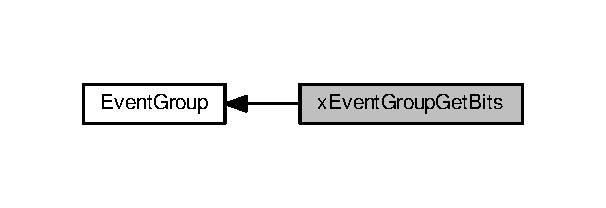
\includegraphics[width=291pt]{group__x_event_group_get_bits}
\end{center}
\end{figure}
\hyperlink{event__groups_8h}{event\+\_\+groups.\+h} 
\begin{DoxyPre}
   EventBits\_t \hyperlink{event__groups_8h_a0ae86f092fb07ccb475ae938f9a12584}{xEventGroupGetBits( EventGroupHandle\_t xEventGroup )};
\end{DoxyPre}


Returns the current value of the bits in an event group. This function cannot be used from an interrupt.


\begin{DoxyParams}{Parameters}
{\em x\+Event\+Group} & The event group being queried.\\
\hline
\end{DoxyParams}
\begin{DoxyReturn}{Returns}
The event group bits at the time \hyperlink{event__groups_8h_a0ae86f092fb07ccb475ae938f9a12584}{x\+Event\+Group\+Get\+Bits()} was called. 
\end{DoxyReturn}
